\documentclass[10pt,a4paper, margin=1in]{article}
\usepackage{fullpage}
\usepackage{amsfonts, amsmath, pifont}
\usepackage{amsthm}
\usepackage{graphicx}
\usepackage{pgfplots}
\usepackage{tikz}
\usepackage{float}
\usepackage{tkz-euclide}
\pgfplotsset{compat=1.13}

\usetikzlibrary{angles,quotes}


\begin{filecontents}{q2a_1.dat}
 n   xn
 0    0
 1    1
 2    0
 3    -1
\end{filecontents}

\begin{filecontents}{q2b.dat}
 n   xn
 0    0
 1    1
 2    -1
 3    1
 4    -1
 5    1
 6    -1
 7    1
 8    -1
 9    1
\end{filecontents}

\begin{filecontents}{q3a.dat}
 n   xn
 -3   6
 0    2
 1    3
 4	  1	 
\end{filecontents}

\begin{filecontents}{q3b.dat}
 n   xn
 -2   1
 -1   2
 0    2
 1	  1	 
\end{filecontents}

\begin{filecontents}{q5b.dat}
 n   xn
 -1   1
 -0   -2
 1    1
\end{filecontents}

\usepackage{geometry}
 \geometry{
 a4paper,
 total={210mm,297mm},
 left=10mm,
 right=10mm,
 top=10mm,
 bottom=10mm,
 }
 % Write both of your names here. Fill exxxxxxx with your ceng mail address.
 \author{
  BAŞŞİMŞEK, Orçun\\
  \texttt{e2098804@ceng.metu.edu.tr}
  \and
  TONKAL, Özlem\\
  \texttt{e1881531@ceng.metu.edu.tr}
}
\title{CENG 384 - Signals and Systems for Computer Engineers \\
Spring 2021 \\
Homework 2}
\begin{document}
\maketitle



\noindent\rule{19cm}{1.2pt}

\begin{enumerate}

\item %write the solution of q1
    \begin{enumerate}
    % Write your solutions in the following items.
    \item %write the solution of q1a
    $-6y(t) - 5y'(t) + x'(t) = y''(t)$
    \item %write the solution of q1b
    We need to form general solution for $y(t)$ by finding homogeneous solution $y_h(t)$ and $y_p(t)$ for given particular input. After that, we need to sum according to superposition property. \\
    
    $y(t) = y_h(t) + y_p(t)$ \\
    
    For homogeneous solution, we assume that the system has no input (i.e. $x(t) = 0$) and we can benefit from exponential function like $y_h(t) = C e^{\alpha t}$. \\
    Since $x(t) = 0$, \ $x'(t) = 0$ also. Therefore our equation for homogeneous solution will be: \\
    \\
    $y''(t) + 5y'(t) + 6y(t) = 0$  \\
    
    Now, we need to put $y(t) = C e^{\alpha t}$ into above equation by finding first and second derivative of it. \\
    $y'(t) = C \alpha e^{\alpha t}$ \\
    $y''(t) = C \alpha^2 e^{\alpha t}$ \\
    \\
    $C \alpha^2 e^{\alpha t} + 5 C \alpha e^{\alpha t} + 6 C e^{\alpha t} = 0$ \\
    $C e^{\alpha t} (\alpha^2 + 5 \alpha + 6) = 0$ \\
    When we equate $(\alpha^2 + 5 \alpha + 6)$ to zero, there are two $\alpha$ values. These are: \\
    $\alpha_1 = -2$ and $\alpha_2 = -3$. Therefore, our homogeneous solution will be: \\
    \\
    $y_h(t) = C_1 e^{-2 t} + C_2 e^{-3 t}$ [equation no. 1] \\
    \\
    Now, we also need to find particular solution $y_p(t)$ for given particular input. Here, we can use the definition of linearity. Since the given system is LTI, any input-output pair of this system should be proportional since superposition property is hold. In other words, since given particular input is $x(t) = (e^{-t} + e^{-4t})u(t)$, we can say that: \\
    \\
    $y_p(t) = A e^{-t} + B e^{-4t}$ \\
    \\
    Now, similar to homogeneous solution case, we need to find derivatives of $y_p(t)$ and put them on the given equation again. \\
    
    $y_p'(t) = -A e^{-t} -4B e^{-4t}$ \\
    $y_p''(t) = A e^{-t} + 16B e^{-4t}$ \\
    Also this time, for this particular solution, we need $x'(t) = (-e^{-t} -4 e^{-4t})$ 
    \\
    Now, put them on the main equation from part (a): \\
    \\
    $-6y(t) - 5y'(t) + x'(t) = y''(t)$ \\
    $x'(t) = y''(t) + 5y'(t) + 6y(t)$ \\
    \\
    $(-e^{-t} -4 e^{-4t}) =  A e^{-t} + 16B e^{-4t} + 5(-A e^{-t} -4B e^{-4t}) + 6(A e^{-t} + B e^{-4t})$ \\
    $-e^{-t} -4 e^{-4t} =  A e^{-t} + 16B e^{-4t} -5A e^{-t} -20B e^{-4t} + 6A e^{-t} + 6B e^{-4t}$ \\
    $-e^{-t} -4 e^{-4t} =  2A e^{-t} + 2B e^{-4t} $ \\
    Hence, \\
    $2A = -1$, \ $A = - \frac{1}{2}$ \\
    $2B = -4$, \ $B = -2$ \\
    \\
    \\
    By substituting A and B on $y_p(t) = A e^{-t} + B e^{-4t}$ \\
    We get, \\
    $y_p(t) = - \frac{1}{2}e^{-t} -2 e^{-4t}$ [equation no. 2] \\
    \\
    Now, we need to form general solution by adding homogeneous and particular solutions (from equation no. 1 and equation no. 2). \\
    $y(t) = y_h(t) + y_p(t)$ \\
    \\
    $y(t) = C_1 e^{-2 t} + C_2 e^{-3 t} - \frac{1}{2}e^{-t} -2 e^{-4t} $  [equation no. 3]\\
    \\
    Since the system is initially at rest, we know that $y(0) = y'(0) = 0$. Therefore, we can use these initial conditions to find constants $C_1$ and $C_2$. \\
    \\
    $y(0) = C_1 + C_2 - \frac{1}{2} -2 = 0$ \\
    $ C_1 + C_2 =  \frac{5}{2}$ [equation no. 4] \\
    \\
    $y'(t) = -2C_1 e^{-2 t} -3C_2 e^{-3 t} + \frac{1}{2}e^{-t} +8 e^{-4t}$ \\
    $y'(0) = -2C_1 -3C_2 + \frac{1}{2} +8 = 0$ \\
    $2C_1 + 3C_2 = \frac{17}{2}$ [equation no. 5] \\
    \\
    By solving [equation no. 4] and [equation no. 5] together, we get: \\
    $C_1 = -1$ and $C_2 = \frac{7}{2}$ \\
    When we put these values into [equation no. 3], we finally reach the result as: \\
    \\
    $y(t) = [- e^{-2 t} + \frac{7}{2} e^{-3 t} - \frac{1}{2}e^{-t} -2 e^{-4t}]u(t) $
    
    
    
    \end{enumerate}

\item %write the solution of q2
    \begin{enumerate}
    % Write your solutions in the following items.
    \item %write the solution of q2a
    We know that the system is LTI. When we analyze graph of $x[n]$, it is easily seen that input $x_1[n]$ is the summation of $x[n]$ and its 2 unit shifted to the left and then multiplicated by 1 version. In other words: \\
     \[ x_1[n] = x[n] - x[n-2] \]
     
     Here, since the system is time invariance, time shift at the input reflects same time shift at the output. In other words: \\
     \[ x[n-2] \ \ gives \ \ y[n-2] \]
     
     Also, we already know that: \\
     \[ x[n] \ \ gives \ \ y[n] \]
     
     Therefore, to create input $x_1[n] = x[n] - x[n-2]$, we can use superposition property since the system is linear. \\
     \[ x_1[n] = x[n] - x[n-2] \ \ gives \ \ y_1[n] = y[n] - y[n-2] \]
     
     As a result, according to given figure of $y[n]$, we can reach $y_1[n]$ as follows: \\
     
    
    \begin{figure} [h!]
    \centering
    \begin{tikzpicture}[scale=0.8] 
      \begin{axis}[
          axis lines=middle,
          xlabel={$n$},
          ylabel={$\boldsymbol{y_1[n]}$},
          xtick={ -1, 0, 1, 2, 3,4},
          ytick={-2, -1, ..., 2},
          ymin=-2, ymax=2,
          xmin=-1, xmax=4,
          every axis x label/.style={at={(ticklabel* cs:1.05)}, anchor=west,},
          every axis y label/.style={at={(ticklabel* cs:1.05)}, anchor=south,},
          grid,
        ]
        \addplot [ycomb, black, thick, mark=*] table [x={n}, y={xn}] {q2a_1.dat};
      \end{axis}
    \end{tikzpicture}
    \caption{$n$ vs. $y_1[n]$.}
    \label{fig:q2a_1}
\end{figure}
    \item %write the solution of q2b
    We know that for discrete LTI systems, convolution summation is: \\
    \[ y[n] = \sum_{k= -\infty}^{\infty} x[k]h[n-k] \]
    Here, we can simply use given input-output pair's values to reach impulse response $h[n]$. \\
    Firstly, when we put $n=0$:
     \[ y[0] = 0 =  \sum_{k= -\infty}^{\infty} x[k]h[-k] = x[0]h[0] + x[1]h[-1]\]
     \[ = h[0] + h[-1] \]
     Since the system is initially at rest, for any response of this system: $y[n] = 0$  when $n<0$. Thus, for also impulse response, this condition is still valid. Therefore, $h[-1] = 0$. \\
     Since we found $h[0] + h[-1] = 0$ at above. $h[0] = 0$ also. \\
     When we continue to write the convolution summation terms for other $n$ values:
     \[ when \ n=1: \ y[1] = 1 = \sum_{k= -\infty}^{\infty} x[k]h[1-k] = x[0]h[1] + x[1]h[0]  \rightarrow h[1] = 1 \]
     \[ when \ n=2: \ y[2] = 0 = \sum_{k= -\infty}^{\infty} x[k]h[2-k] = x[0]h[2] + x[1]h[1]  \rightarrow h[2]+h[1] = 0 \rightarrow h[2] = -1 \]
     \[ when \ n=3: \ y[3] = 0 = \sum_{k= -\infty}^{\infty} x[k]h[3-k] = x[0]h[3] + x[1]h[2]  \rightarrow h[3]+h[2] = 0 \rightarrow h[3] = 1 \]
     \[ when \ n=4: \ y[4] = 0 = \sum_{k= -\infty}^{\infty} x[k]h[4-k] = x[0]h[4] + x[1]h[3]  \rightarrow h[4]+h[3] = 0 \rightarrow h[4] = -1 \]
     
     Actually, we reached the pattern here for impulse response $h[n]$. It is $h[n] = 1$ when n is odd and $h[n] = -1$ when n is even (except $h[0]=0$). And, it continues forever with this pattern. Thus, it is infinite impulse response. We already know the unit step function whose value is always $1$ when $n \geq 0$. Therefore, we can write $h[n]$ in terms of it as: \\
      \[ h[n] = (-1)^{n-1}u[n-1]\]
      
      \begin{figure} [h!]
    \centering
    \begin{tikzpicture}[scale=0.8] 
      \begin{axis}[
          axis lines=middle,
          xlabel={$n$},
          ylabel={$\boldsymbol{h[n]}$},
          xtick={ -1, 0, 1, 2, 3,4,5,6,7,8,9},
          ytick={-2, -1, ..., 2},
          ymin=-2, ymax=2,
          xmin=-1, xmax=9,
          every axis x label/.style={at={(ticklabel* cs:1.05)}, anchor=west,},
          every axis y label/.style={at={(ticklabel* cs:1.05)}, anchor=south,},
          grid,
        ]
        \addplot [ycomb, black, thick, mark=*] table [x={n}, y={xn}] {q2b.dat};
      \end{axis}
    \end{tikzpicture}
    \caption{$n$ vs. $h[n]$. (n continues towards infinity with this pattern)}
    \label{fig:q2b_1}
\end{figure}
    \item %write the solution of q2c
    From part (b), we have already found $h[n] = (-1)^{n-1}u[n-1]$. We can also write it in terms of unit impulse functions as follows:
     \[ h[n] = \delta[n-1] - \delta[n-2] + \delta[n-3] - \delta[n-4] + \delta[n-5] - \delta[n-6] ... \]
     Hence, with $y[n] = x[n] * h[n]$, we can easily say that:
     \[ y[n] =  x[n-1] - x[n-2] + x[n-3] - x[n-4] + x[n-5] - x[n-6] ... \]
     If we also evaluate $y[n-1]$ and add it to $y[n]$,  we can reach more compact equation as follows: \\
    \[ y[n-1] = x[n-2] - x[n-3] + x[n-4] - x[n-5] + x[n-6] - x[n-7] ... \]
     \[  y[n] =  x[n-1] - x[n-2] + x[n-3] - x[n-4] + x[n-5] - x[n-6] ...\]
     \[ y[n] + y[n-1] = x[n-1] \ \ \ (RESULT \ of \ 2.c) \] 
    \item %write the solution of q2d
    
    \tikzset{%
		block/.style    = {draw, thick, rectangle, minimum height = 3em,
			minimum width = 3em},
		sum/.style      = {draw, circle, node distance = 2cm}, % Adder
		input/.style    = {coordinate}, % Input
		output/.style   = {coordinate} % Output
	}
	% Defining string as labels of certain blocks.
	\newcommand{\suma}{\Large$+$}
	\newcommand{\delay}{$D$}
	\newcommand{\derv}{\huge$\frac{d}{dt}$}
	
	\begin{figure} [h!]
	\begin{tikzpicture}[auto, thick, node distance=2cm, >=triangle 45]
	\draw
	% Drawing the blocks of first filter :
	node at (0, 0) [input] (inp) {\Large \textopenbullet}
	node [block, right of=inp] (int1) {\delay}
	node [sum, right of=int1] (sum) {\suma}
	node [output, right of=sum] (out1) {}
	node [output, right of=out1] (out) {}
	node [output, right of=out] (out2) {\Large \textopenbullet}
	node [output, below of=out] (temp1) {}
	node [block, left of=temp1] (int3) {\delay}
	node [output, left of=int3] (temp3) {}
	node [output, below of=sum] (temp2) {}
	;
	\draw[->](inp) -- node{$x[n]$} (int1);
	\draw[->](int1) -- (sum);
	\draw[-](sum) -- (out1);
	\draw[-](out1) -- (out);
	\draw[->](out) -- node{$y[n]$} (out2);
	\draw[-](out) -- (temp1);
	\draw[-](temp1) -- (int3);
	\draw[-](int3) -- (temp3);
	\draw[->](temp2) -- node{$-$} (sum);
	\end{tikzpicture}
	\end{figure}	
    \end{enumerate}

\item %write the solution of q3  
    \begin{enumerate}
    % Write your solutions in the following items.
    \item %write the solution of q3a
    $y[n] = x[n] * h[n]$ \\
    \\
    By using distributive property: \\
    $y[n] = x[n] * \delta[n-1] + x[n] * 3\delta[n+2]$ \\
    \\
    By using sampling property: \\
    $y[n] = x[n-1] + 3x[n+2]$ \\
    \\
    Hence, \\
    $y[n] = \delta[n-4] +3\delta[n-1] + 2\delta[n] +6\delta[n+3] $ \\
    \\
    \\
    Graphic of $y[n]$ is as follows: \\
    
    \begin{figure} [h!]
    \centering
    \begin{tikzpicture}[scale=0.9] 
      \begin{axis}[
          axis lines=middle,
          xlabel={$n$},
          ylabel={$\boldsymbol{y[n]}$},
          xtick={-5, -4, -3, -2, -1, 0, 1,2,3,4,5},
          ytick={-2, -1, ..., 7},
          ymin=-2, ymax=7,
          xmin=-5, xmax=5,
          every axis x label/.style={at={(ticklabel* cs:1.05)}, anchor=west,},
          every axis y label/.style={at={(ticklabel* cs:1.05)}, anchor=south,},
          grid,
        ]
        \addplot [ycomb, black, thick, mark=*] table [x={n}, y={xn}] {q3a.dat};
      \end{axis}
    \end{tikzpicture}
    \caption{$n$ vs. $y[n]$.}
    \label{fig:q3_a}
\end{figure} 
    \item %write the solution of q3b
    
    \[x[n] = u[n+3] - u[n]\]
    \[x[n] = \sum_{k=0}^{\infty} \delta[n+3-k] - \sum_{k=0}^{\infty} \delta[n-k] \]
    \[x[n] =\delta[n+3] + \delta[n+2] + \delta[n+1] \] \\
    On the other hand, for $h[n]$: \\
    \[h[n] = u[n-1] - u[n-3]\]
    \[h[n] = \sum_{k=0}^{\infty} \delta[n-1-k] - \sum_{k=0}^{\infty} \delta[n-3-k] \]
    \[h[n] =\delta[n-1] + \delta[n-2] \] \\
    Now, for convolution: \\
    $y[n] = x[n] * h[n]$ \\
    \\
    By using distributive property: \\
    $y[n] = x[n] * \delta[n-1] + x[n] * \delta[n-2]$ \\
    \\
    By using sampling property: \\
    $y[n] = x[n-1] + x[n-2]$ \\
    \\
    Hence, \\
    $y[n] = \delta[n+2] +2\delta[n+1] + 2\delta[n] +\delta[n-1] $ \\
    \\
    \\
    Graphic of $y[n]$ is as follows: \\
    
    \begin{figure} [h!]
    \centering
    \begin{tikzpicture}[scale=0.9] 
      \begin{axis}[
          axis lines=middle,
          xlabel={$n$},
          ylabel={$\boldsymbol{y[n]}$},
          xtick={-3,-2, -1, 0, 1,2,3},
          ytick={-3, -2, ..., 3},
          ymin=-3, ymax=3,
          xmin=-3, xmax=3,
          every axis x label/.style={at={(ticklabel* cs:1.05)}, anchor=west,},
          every axis y label/.style={at={(ticklabel* cs:1.05)}, anchor=south,},
          grid,
        ]
        \addplot [ycomb, black, thick, mark=*] table [x={n}, y={xn}] {q3b.dat};
      \end{axis}
    \end{tikzpicture}
    \caption{$n$ vs. $y[n]$.}
    \label{fig:q3_b}
\end{figure} 
    \end{enumerate}

\item %write the solution of q4
    \begin{enumerate}
    % Write your solutions in the following items.
    \item %write the solution of q4a
    \[ y(t) =  \int_{- \infty}^{\infty} x(\tau)h(t-\tau) \,d\tau \]
     \[ =  \int_{0}^{t} e^{-2\tau}e^{-3(t-\tau)} \,d\tau \]
     \[ =  e^{-3t} \int_{0}^{t} e^{\tau} \,d\tau \]
     \[ =  e^{-3t} (e^{t}-1) \] \\
     Thus, $y(t) = (e^{-2t} - e^{-3t}) u(t)$ \\
     \\
    \item %write the solution of q4b
    Here, $x(t)$ is simply finite pulse between $t=0$ and $t=2$. In other words, $x(t)$ is: \\
    
    \begin{figure}[H]
    \centering
        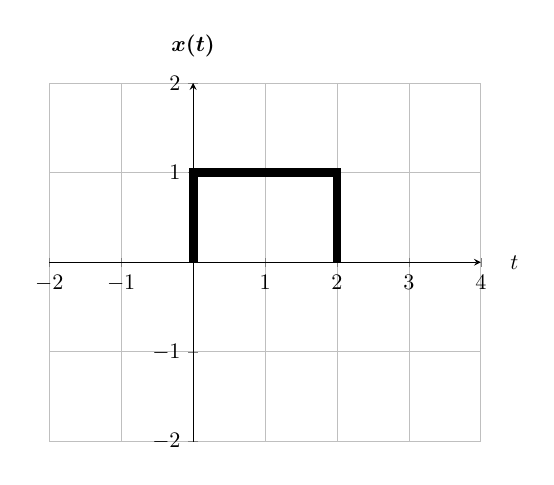
\begin{tikzpicture}[scale=0.8]
           \begin{axis}[
          axis lines=middle,
          xlabel={$t$},
          ylabel={$\boldsymbol{x(t)}$},
          xtick={-2, ..., 4},
          ytick={-2, -1, ..., 2},
          ymin=-2, ymax=2,
          xmin=-2, xmax=4,
          every axis x label/.style={at={(ticklabel* cs:1.05)}, anchor=west,},
          every axis y label/.style={at={(ticklabel* cs:1.05)}, anchor=south,},
          grid,
        ]
           \path[draw,line width=4pt] (0,0) -- (0,1) -- (2,1) -- (2,0);
           \end{axis}
        \end{tikzpicture}
        \caption{$t$ vs. $x(t)$.}
        \label{fig:q4_1}
    \end{figure}
    
    We need to find $x(t-\tau)$ for convolution operation. We first change the variable $t$ to $\tau$, then do time-reverse, and then shift by $t$. The resulting graph is as follows: \\
    
    \begin{figure}[H]
    \centering
        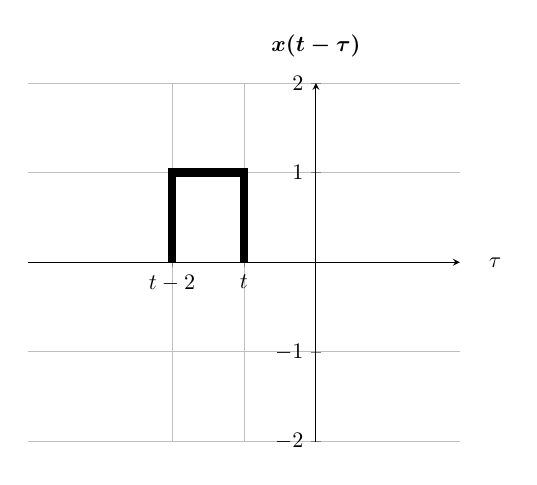
\begin{tikzpicture}[scale=0.8]
           \begin{axis}[
          axis lines=middle,
          xlabel={$\tau$},
          ylabel={$\boldsymbol{x(t-\tau)}$},
          xtick={-2,-1},
          xticklabels={$t-2$, $t$},
          ytick={-2, -1, ..., 2},
          ymin=-2, ymax=2,
          xmin=-4, xmax=2,
          every axis x label/.style={at={(ticklabel* cs:1.05)}, anchor=west,},
          every axis y label/.style={at={(ticklabel* cs:1.05)}, anchor=south,},
          grid,
        ]
           \path[draw,line width=4pt] (-2,0) -- (-2,1) -- (-1,1) -- (-1,0);
           \end{axis}
        \end{tikzpicture}
        \caption{$\tau$ vs. $x(t-\tau)$.}
        \label{fig:q4_2}
    \end{figure}
    
    We also need to $h(\tau) = e^{2\tau}u(\tau)$. Its graph is also as follows: \\
    
 \begin{figure}[H]
    \centering   
\begin{tikzpicture}
\begin{axis}[
        xlabel={$\tau$},
        ylabel={$h(\tau)$},
        axis lines=center,
        xmin=0,xmax=4.9,
        ymin=0,ymax=4.9,
        ytick={1},
        yticklabels={1}
]

\addplot +[mark=none,smooth] {e^(x)};
\draw [dashed] (0,1) -- (\pgfkeysvalueof{/pgfplots/xmax},1);

\end{axis}
\end{tikzpicture}
\caption{$\tau$ vs. $h(\tau)$.}
        \label{fig:q4_3}
\end{figure}

Here, when we analyze graphs, there are 3 different cases according to values of $t$. \\
First case: When $t \leq 0$, there is no overlap between functions $x(t-\tau)$ and $h(\tau)$ as seen on the figures. Therefore, \\
$ y(t) =  \int_{- \infty}^{\infty} x(t-\tau)h(\tau) \,d\tau = 0 $ \\
\\
\\
\\
Second case: When $t>0$ and $t-2 \leq 0$, overlap between functions $x(t-\tau)$ and $h(\tau)$ starts to occur. Therefore, \\
 \[y(t) =  \int_{- \infty}^{\infty} x(t-\tau)h(\tau) \,d\tau   \]
 \[=  \int_{0}^{t} x(t-\tau)h(\tau) \,d\tau   \]
 \[=  \int_{0}^{t} 1 \times e^{2\tau} \,d\tau   \]
 \[=  |_0^t \ \ \frac{e^{2\tau}}{2}   \]
 \[=  \frac{e^{2t} - 1}{2}  \]
 
 Third case: When $t-2>0$, overlap between functions $x(t-\tau)$ and $h(\tau)$ still continues. Therefore, \\
 \[y(t) =  \int_{- \infty}^{\infty} x(t-\tau)h(\tau) \,d\tau   \]
 \[=  \int_{t-2}^{t} x(t-\tau)h(\tau) \,d\tau   \]
 \[=  \int_{t-2}^{t} 1 \times e^{2\tau} \,d\tau   \]
 \[=  |_{t-2}^t \ \ \frac{e^{2\tau}}{2}   \]
 \[=  \frac{e^{2t} - e^{2t-4}}{2}  \]
 \[=  \frac{e^{2t}(1 - e^{-4})}{2}  \]
 
 When we combine these three cases, we get $y(t)$ as: \\
 
  \[y(t) = \begin{cases} 
      0 & t \leq 0 \\
      \frac{e^{2t} - 1}{2} &  0 < t \leq 2 \\
      \frac{e^{2t}(1 - e^{-4})}{2} & t > 2 
   \end{cases}
\]

    
    \end{enumerate}

\item %write the solution of q5
    \begin{enumerate}
    % Write your solutions in the following items.
    \item %write the solution of q5a
    \[ h[n] = s[n] - s[n-1] \]
    \[ = nu[n] - (n-1)u[n-1] \]
    \[ = nu[n] - nu[n-1] + u[n-1] \]
    \[ = n(u[n]-u[n-1]) + u[n-1] \]
    \[ = n\delta[n] + u[n-1] \]
    Since $n\delta[n]$ term is 0, impulse response is: \\
    \[ h[n] = u[n-1] \]
    \item %write the solution of q5b
    We can use convolution summation to find given output $y[n] = \delta[n] - \delta[n-1]$:
    \[ y[n] = \sum_{k= -\infty}^{\infty} x[k]h[n-k] \]
    We have already found impulse response, so put it on this equation:
    \[ y[n] = \delta[n] - \delta[n-1] = \sum_{k= -\infty}^{\infty} x[k]u[n-k-1] \]
    Since left-hand side of the equation contains unit impulse functions, on the right-hand side we can write $u[n-k-1]$ in terms of unit impulse functions as well.
    \[ y[n] = \delta[n] - \delta[n-1] = \sum_{k= -\infty}^{\infty} x[k]\{\delta[n-k-1] + \delta[n-k-2] + \delta[n-k-3] + \delta[n-k-4] + ...\} \]
    For right-hand side of this equation, when we write the terms of summation a little bit:
    \[ when \ k=-1: \ x[-1]\{\delta[n] + \delta[n-1] + \delta[n-2] + \delta[n-3] + ...\}   \]
    \[ when \ k=0: \ x[0]\{\delta[n-1] + \delta[n-2] + \delta[n-3] + \delta[n-4] + ...\}   \]
    \[ when \ k=1: \ x[1]\{\delta[n-2] + \delta[n-3] + \delta[n-4] + \delta[n-5] + ...\}   \]
    Since we had $y[n] = \delta[n] - \delta[n-1]$ on left-hand side, we need to have $x[-1] = 1$, $x[0] = -2$, $x[1] = 1$ to obtain same result on right-hand side. Hence, the graph of $x[n]$ is as follows: \\
    \\
$x[n] = \delta[n+1] -2\delta[n] + \delta[n-1]$ (RESULT of 5.b)    
    \begin{figure} [H]
    \centering
    \begin{tikzpicture}[scale=0.9] 
      \begin{axis}[
          axis lines=middle,
          xlabel={$n$},
          ylabel={$\boldsymbol{x[n]}$},
          xtick={-3,-2, -1, 0, 1,2,3},
          ytick={-3, -2, ..., 3},
          ymin=-3, ymax=3,
          xmin=-3, xmax=3,
          every axis x label/.style={at={(ticklabel* cs:1.05)}, anchor=west,},
          every axis y label/.style={at={(ticklabel* cs:1.05)}, anchor=south,},
          grid,
        ]
        \addplot [ycomb, black, thick, mark=*] table [x={n}, y={xn}] {q5b.dat};
      \end{axis}
    \end{tikzpicture}
    \caption{$n$ vs. $x[n]$.}
    \label{fig:q5_b}
\end{figure} 
    
     
    \item %write the solution of q5c
    In part (a), we found $h[n] = u[n-1]$ which is also equal to: 
    \[ h[n] = \delta[n-1] + \delta[n-2]+ \delta[n-3]+ \delta[n-4]+ ... \]
    Hence, with $y[n] = x[n] * h[n]$, we can easily say that:
    
    \[ y[n] = x[n-1] + x[n-2]+ x[n-3]+ x[n-4]+... \]
    If we also evaluate $y[n+1]$ and subtract $y[n]$ from it,  we can reach more compact equation as follows: \\
    \[ -y[n] = -x[n-1] - x[n-2] - x[n-3] - x[n-4] - ... \]
    \[ y[n+1] = x[n] + x[n-1]+ x[n-2]+ x[n-3]+... \]
    \[ y[n+1] - y[n] = x[n] \ \ \ (RESULT \ of \ 5.c) \]     
    \end{enumerate}

\item %write the solution of q6

We know that $h(t) = \frac{ds(t)}{dt}$. Therefore, \\

$\frac{ds(t)}{dt} = tu(t)$ \\
\\
$h(t) = tu(t)$ \\
Now, we can use this impulse response for convolution operation to find $y(t)$. \\
As an input, we already have $x(t) = e^{-t}u(t)$ \\
Also, since both $h(t)$ and $x(t)$ are multiplied with unit step function, there is no overlap between them when $t<0$. Therefore, when $t<0$, $y(t) = 0$.\\
When $t \geq 0$:
 \[y(t) =  \int_{- \infty}^{\infty} x(\tau)h(t-\tau) \,d\tau   \]
 \[ =  \int_{0}^{t} e^{-\tau}(t-\tau) \,d\tau   \]
 \[ =  \int_{0}^{t} te^{-\tau} \,d\tau - \int_{0}^{t} \tau e^{-\tau} \,d\tau  \]
 \[ =  t \int_{0}^{t} e^{-\tau} \,d\tau - \int_{0}^{t} \tau e^{-\tau} \,d\tau  \]
  \[ =  t  (|_0^t -e^{-\tau}) - \int_{0}^{t} \tau e^{-\tau} \,d\tau  \]
\[ =  t  (1 -e^{-t}) - \int_{0}^{t} \tau e^{-\tau} \,d\tau  \]
\[ =    (t -te^{-t}) - \int_{0}^{t} \tau e^{-\tau} \,d\tau  \ [eq.1] \]  \\
Now, for this integral $\int_{0}^{t} \tau e^{-\tau} \,d\tau$, we need to use integration by parts method. \\

$\tau = u$ implies that $d\tau = du$ \\
$\int  e^{-\tau} \,d\tau = dv$ implies that $-e^{-\tau} = v$ 
\[ \int_{0}^{t} \tau e^{-\tau} \,d\tau = |_0^t uv - \int_0^t \, vdu \]
\[  = |_0^t \tau (-e^{-\tau}) - \int_0^t -e^{-\tau} \,d\tau \]
\[  = (-te^{-t}) + \int_0^t e^{-\tau} \,d\tau \]
\[  = -te^{-t} + |_0^t (-e^{-\tau}) \]
\[  = -te^{-t} + (1-e^{-t}) \] \\

When we put this result to its place above on [eq.1]:

\[y(t) = (t -te^{-t}) - (-te^{-t} + 1-e^{-t}) \]
\[y(t) = e^{-t} +t -1\]


\item %write the solution of q7
    \begin{enumerate}
    % Write your solutions in the following items.
    \item %write the solution of q7a
    $x(t) * u(t) * \delta(t-3) - x(t) * u(t) * \delta(t-5) =y(t)$ \\
    \\
    When we put $\delta(t)$ as an input in this system, we will get impulse response $h(t)$: \\
    \\
    $\delta(t) * u(t) * \delta(t-3) - \delta(t) * u(t) * \delta(t-5) =h(t)$ \\
    \\
    Here, we know that $\delta(t) * u(t) = u(t)$ according to sampling property. Therefore, \\
    \\
    $u(t) * \delta(t-3) - u(t) * \delta(t-5) =h(t)$ \\
    \\
    Again, $u(t) * \delta(t-3) = u(t-3)$ and $u(t) * \delta(t-5) = u(t-5)$ according to sampling property. Therefore, impulse response of this system is: \\
    \\
     $h(t) = u(t-3) - u(t-5)$ 
     \\
     
     \begin{figure}[H]
    \centering
        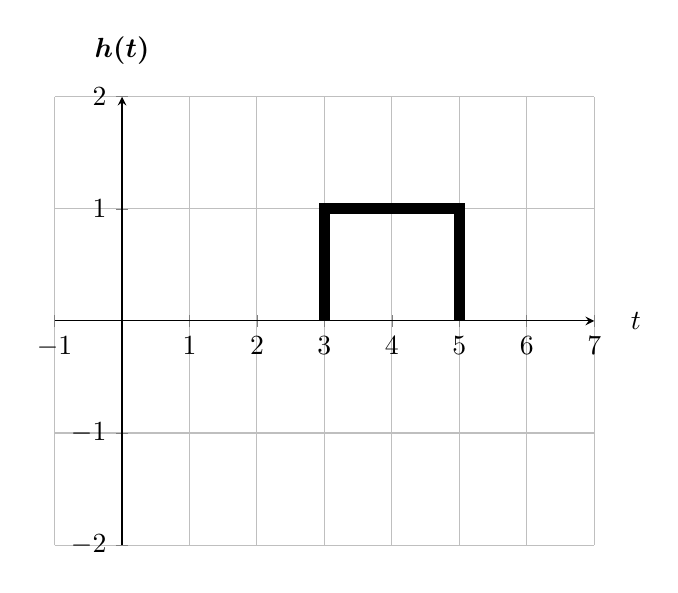
\begin{tikzpicture}[scale=1.0]
           \begin{axis}[
          axis lines=middle,
          xlabel={$t$},
          ylabel={$\boldsymbol{h(t)}$},
          xtick={-1,0,1,2,3,4,5,6,7},
          ytick={-2, -1, ..., 2},
          ymin=-2, ymax=2,
          xmin=-1, xmax=7,
          every axis x label/.style={at={(ticklabel* cs:1.05)}, anchor=west,},
          every axis y label/.style={at={(ticklabel* cs:1.05)}, anchor=south,},
          grid,
        ]
           \path[draw,line width=4pt] (3,0) -- (3,1) -- (5,1) -- (5,0);
           \end{axis}
        \end{tikzpicture}
        \caption{$t$ vs. $h(t)$.}
        \label{fig:q7_a}
    \end{figure}
    
    \item %write the solution of q7b
	
	\[ y(t) =  \int_{- \infty}^{\infty} x(\tau)h(t-\tau) \,d\tau \]  
	\\
	\\
	\\
	
	Here, since we already know $h(t)$ from part (a), firstly, we can plot the graph of $h(t-\tau)$ easily. \\
	\\
	\\
	
	
	\begin{figure}[H]
    \centering
        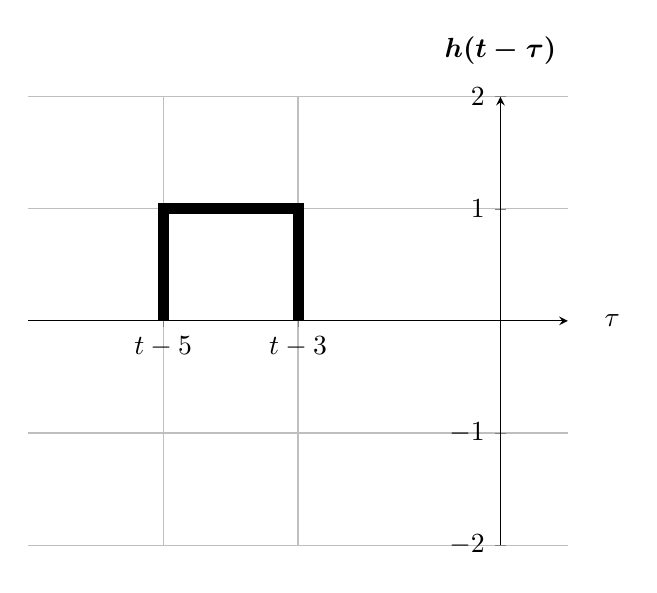
\begin{tikzpicture}[scale=1.0]
           \begin{axis}[
          axis lines=middle,
          xlabel={$\tau$},
          ylabel={$\boldsymbol{h(t-\tau)}$},
          xtick={-5,-3},
          xticklabels={$t-5$, $t-3$},
          ytick={-2, -1, ..., 2},
          ymin=-2, ymax=2,
          xmin=-7, xmax=1,
          every axis x label/.style={at={(ticklabel* cs:1.05)}, anchor=west,},
          every axis y label/.style={at={(ticklabel* cs:1.05)}, anchor=south,},
          grid,
        ]
           \path[draw,line width=4pt] (-5,0) -- (-5,1) -- (-3,1) -- (-3,0);
           \end{axis}
        \end{tikzpicture}
        \caption{$\tau$ vs. $h(t-\tau)$.}
        \label{fig:q7_b}
    \end{figure}
    
    
    We also need to $x(\tau) = e^{-3\tau}u(\tau)$. Its graph is also as follows: \\
    
 \begin{figure}[H]
    \centering   
\begin{tikzpicture}
\begin{axis}[
        xlabel={$\tau$},
        ylabel={$x(\tau)$},
        axis lines=center,
        xmin=0,xmax=2.9,
        ymin=0,ymax=2.9,
        ytick={1},
        yticklabels={1}
]

\addplot +[mark=none,smooth] {e^(-x)};
\draw [dashed] (0,1) -- (\pgfkeysvalueof{/pgfplots/xmax},1);

\end{axis}
\end{tikzpicture}
\caption{$\tau$ vs. $x(\tau)$.}
        \label{fig:q4_3}
\end{figure}

Here, when we analyze graphs, there are 3 different cases according to values of $t$. \\
First case: When $t-3 \leq 0$, there is no overlap between functions $x(t-\tau)$ and $h(\tau)$ as seen on the figures. Therefore, \\
$ y(t) =  \int_{- \infty}^{\infty} x(\tau)h(t-\tau) \,d\tau = 0 $ \\
\\
\\
\\
Second case: When $t-3>0$ and $t-5 \leq 0$, overlap between functions $x(t-\tau)$ and $h(\tau)$ starts to occur. Therefore, \\
 \[y(t) =  \int_{- \infty}^{\infty} x(\tau)h(t-\tau) \,d\tau   \]
 \[=  \int_{0}^{t-3} x(\tau)h(t-\tau) \,d\tau   \]
 \[=  \int_{0}^{t-3} e^{-3\tau} \times 1 \,d\tau   \]
 \[=  |_0^{t-3} \ \ \frac{e^{-3\tau}}{-3}   \]
 \[=  \frac{1- e^{-3t+9}}{3}  \]
 
 
 Third case: When $t-5>0$, overlap between functions $x(t-\tau)$ and $h(\tau)$ still continues. Therefore, \\
 \[y(t) =  \int_{- \infty}^{\infty} x(\tau)h(t-\tau) \,d\tau   \]
 \[=  \int_{t-5}^{t-3} x(\tau)h(t-\tau) \,d\tau   \]
 \[=  \int_{t-5}^{t-3} e^{-3\tau} \times 1 \,d\tau   \]
 \[=  |_{t-5}^{t-3} \ \ \frac{e^{-3\tau}}{-3}   \]
 \[=  \frac{e^{-3t+15} - e^{-3t+9}}{3}  \]
 \[=  \frac{e^{-3t+9} (e^{6} - 1)}{3}  \]
 
 When we combine these three cases, we get $y(t)$ as: \\
 
  \[y(t) = \begin{cases} 
      0 & t \leq 3 \\
      \frac{1- e^{-3t+9}}{3} &  3 < t \leq 5 \\
      \frac{e^{-3t+9} (e^{6} - 1)}{3} & t > 5 
   \end{cases}
\]
	 \\
    \item %write the solution of q7c
    We have already found $h(t) = u(t-3) - u(t-5)$. Therefore, $\frac{dh(t)}{dt} = \delta(t-3) - \delta(t-5)$ \\
    
    \[ (\frac{dh(t)}{dt}) * x(t) = (\delta(t-3) - \delta(t-5)) * x(t)  \]
    \[ = \delta(t-3) * x(t) - \delta(t-5) * x(t) \]
    \[ = x(t-3) - x(t-5) \]
    \end{enumerate}    

\end{enumerate}
\end{document}

